\chapter{Monte Carlo Methods}
% Our goal is to estimate value functions and find optimal policies. Monte-Carlo methods require only \textit{experience}--sample sequences of states, actions, and rewards from actual or simulated interaction with an environment. 
Monte Carlo methods are a class of computational algorithms that rely on random sampling to obtain numerical results. In the context of reinforcement learning (RL), Monte Carlo methods are often used to estimate the value of states or state-action pairs in a Markov Decision Process (MDP).


\section{Monte Carlo Prediction (Evaluation)}
Recall that the value of a state is the expected return starting from that state. An obvious way to estimate it from experience, then, is simply to average the returns observed after visits to that state. As more returns are observed, the average should converge to the expected value. This idea is the core of Monte Carlo methods. 

\subsection{First Visit vs. Every Visit}
Suppose we wish to estimate $v_\pi(s)$, the value of a state $s$ under policy $\pi$, given a set of episodes obtained by following $\pi$ and passing through $s$. Each occurrence of state $s$ in an episode is called a visit to $s$. 

\paragraph{The first-visit MC} method estimates $v_\pi(s)$ as the average of the returns following first visits to $s$, whereas \textit{the every-visit MC} method averages the returns following all visits to $s$.

\begin{itemize}
	\item First visit MC treats each trajectory as an i.i.d., sample of $v(s)$.
	\item For instance, we have two example episodes, 
		\begin{itemize}
			\item $A, 3\to A, 2\to B, -4\to A, 4\to B, -3$.
			\item $B, -2\to A, 3\to B, -3$.
		\end{itemize} 
	\item Each number next to the states are reward. Let's say discount factor is 1 and we want to compute $V(A)$, then the first visit MC computes a return by summing all the rewards ($G\leftarrow \gamma G + R_{t+1}$) coming after the first visit to the state $A$. Therefore, we can't have more than one summation term for each episode for a state. In sum,
	\begin{itemize}
		\item For the first episode: $3+2-4+4-3=2$.
		\item For the second episode: $3-3=0$.
		\item Thus, $V(A) = (2+0)/2=1$.
		\item It must be noted that if an episode doesn't have an occurrence of `$A$', it won't be considered in the average. Hence if a 3rd episode is given like $B,3\to B,3\to terminate$ existed, still $V(A)=1$.
	\end{itemize}
\end{itemize}

\begin{figure}[h]
	\centering
	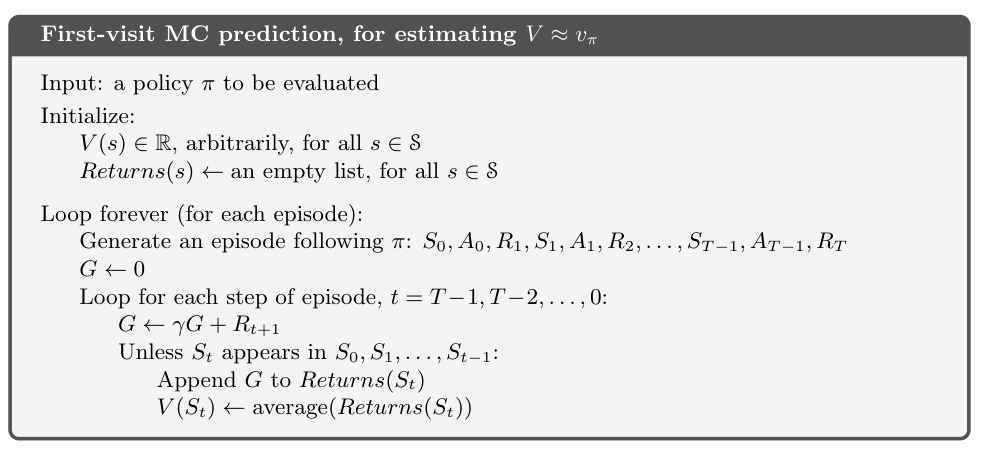
\includegraphics[scale=0.5]{./images/first_visit_mc.png}
	\caption{First-visit MC prediction algorithm.}
	\label{fig:first_visit_mc}
\end{figure}

\paragraph{Every visit MC} method averages the returns following \textbf{all visits} to $s$.
\begin{itemize}
	\item Here, we would be creating a new summation term adding all rewards coming after every occurrence of `$A$'(including that of $A$ as well).
		\begin{itemize}
			\item From 1st episode: $(3+2-4+4-3)+(2-4+4-3)+(4-3)=2-1+1$
			\item From 2nd episode: $(3-3)=0$
			\item As we got 4 summation terms, we will be averaging using $N=4$ \ie
			\item $V(A)=(2-1+1+0)/4=0.5$
		\end{itemize}
\end{itemize}



\section{Monte Carlo Control}
$$\pi_0\xrightarrow{\,E\,} q_{\pi_0} \xrightarrow{\,I\,} \pi_0\xrightarrow{\,E\,} q_{\pi_0}\xrightarrow{\,I\,}\cdots \xrightarrow{\,I\,} \pi_*\xrightarrow{\,E\,} q_{\pi_*},$$
\begin{itemize}
	\item $\pi_0$: arbitrary policy.
	\item Policy improvement is done by making the policy greedy with respect to the current value function (action-value function). 
	\item For any action-value function $q$, the corresponding greedy policy is the one that, for each $s\in \mathcal{S}$, deterministically chooses an action with maximal action-value:
		$$\pi(S) = \argmax_a q(s,a).$$
	\item Policy improvement then can be done by constructing each $\pi_{k+1}$ as the greedy policy with respect to $q_{\pi_k}.$
	\item By \Cref{thrm:policy_improvement}, each $\pi_{k+1}$ is uniformly better than $\pi_k$ or just as good as $\pi_k$.
\end{itemize}

\section{On-Policy vs. Off-Policy}
%Monte Carlo prediction (or evaluation) is used to evaluate the value of a given policy, while Monte Carlo control is for finding the optimal policy when such a policy is not given. There are two categories of MC control:
\begin{itemize}
	\item On-policy: learn about the optimal policy by executing the policy and evaluting and improving it.  
		\begin{itemize}
			\item Learning to be great by itself.
		\end{itemize}
	\item Off-policy: learn about the optimal policy by using data generated by another policy. 
		\begin{itemize}
			\item Learning from others.
		\end{itemize}
\end{itemize}

The more episodes are collected, the better because the estimates of the functions will be. However, there is a problem. If the algorithm for policy improvement always updates the policy greedily, meaning it takes only actions leading to immediate reward, actions and states not on the greedy path will not be sampled sufficiently, and potentially better rewards would stay hidden from the learning process.

Essentially, we are forced to make a choice between making the best decision given the current information or start exploring and finding more information. This is also known as the Exploration vs. Exploitation Dilemma.

We are looking for something like a middle ground between those. Full-on exploration would mean that we would need a lot of time to collect the needed information, and full-on exploitation would make the agent stuck into a local reward maximum. There are two approaches to ensure all actions are sampled sufficiently called on-policy and off-policy methods.



\subsection{On Policy}
On-policy methods solve the exploration vs exploitation dilemma by including randomness in the form of a policy that is soft, meaning that non-greedy actions are selected with some probability. These policies are called $\epsilon$-greedy policies as they select random actions with an $\epsilon$ probability and follow the optimal action with $1-\epsilon$ probability

Since the probability of selecting from the action space randomly is $\epsilon$, the probability of selecting any particular non-optimal (non-greedy) action is $\epsilon/|\mathcal{A}(s)|$. The probability of following the optimal action will always be slightly higher, however, because we have a $1 - \epsilon$ probability of selecting it outright and $\epsilon/ |\mathcal{A}(s)|$ probability of selecting it from sampling the action space \footnote{Since the greedy (or optimal) action can be selected by either 1-$\epsilon$ or $\epsilon/ |\mathcal{A}(s)|$, $a_1=\epsilon/\mathcal{A}(s),a_2=\epsilon/\mathcal{A}(s),\cdots,a_{best}=1-\epsilon+\epsilon/\mathcal{A}(s),a_n = \epsilon/\mathcal{A}(s)$}
$$P(a_t^{*}) = 1 - \epsilon+\epsilon/ |\mathcal{A}(s)|.$$
It is also worth noting that because the optimal action will be sampled more often than the others making on-policy algorithms will generally converge faster but they also have the risk of trapping the agent into a local optimum of the function.

%On-Policy learning algorithms are the algorithms that evaluate and improve the same policy which is being used to select actions. That means we will try to evaluate and improve the same policy that the agent is already using for action selection. In short , [Target Policy == Behavior Policy]. Some examples of On-Policy algorithms are Policy Iteration, Value Iteration, Monte Carlo for On-Policy, Sarsa, etc.

\subsection{Off Policy}

All learning contol methods face a dilemma: They seek to learn action values conditional on subsequent \textit{optimal} behavior, but they need to behave non-optimally in order to explore all actions (to find the optimal actions). How can they learn about the optimal policy while behaving according to an exploratory policy? The on-policy approach in the preceding section is actually a compromise. It learns action values not for the optimal policy, but for a near-optimal policy that still explores. A more straightforward approach is to use two policies, one that is learned about and that becomes the optimal policy, and one that is more exploratory and is used to generate behavior. The policy being learned about is called the \textit{target policy}, and the policy used to generate behavior is called the \textit{behavior policy}. In this case we say that learning is from data ``off'' the target policy, and the overall process is termed \textit{off-policy learning}.

Given a starting state $S_t$, the probability of the subsequent state-action trajectory, $A_t, S_{t+1}, A_{t+1},\cdots,S_T$, occuring under any policy $\pi$ is 
\begin{align*}
	P(A_t, S_{t+1}, A_{t+1},\cdots,S_T)&= \pi(A_t|S_t)p(S_{t+1}|S_t,A_t)\pi(A_{t+1}|S_{t+1})\cdots(S_T|S_{T-1},A_{T-1})\\ 
	&= \prod_{k=t}^{T-1}\pi(A_k|S_k)p(S_{k+1}|S_k,A_k),
\end{align*}
where $p$ here is the state-transition probability function. Thus, the relative probability of the trajectory under the target and behavior policies is 

\begin{align*}
	\rho_{t:T-1} &=  \frac{\prod_{k=t}^{T-1}\pi(A_k|S_k)p(S_{k+1}|S_k,A_k)}{ \prod_{k=t}^{T-1}b(A_k|S_k)p(S_{k+1}|S_k,A_k)}\\
	&= \prod_{k=t}^{T-1}\frac{\pi(A_k|S_k)}{b(A_k|S_k)}.
	% \label{eq:importance_sampling_ratio}
\end{align*}
The importance sampling ratio ends up depending only on the two polices and the sequence, not on the MDP (state-transition probability).

Recall that we wish to estimate the expected returns under the target policy, but all we have are returns $G_t$ from the behavior policy, which reulsts in 
\begin{align*}
	\mathbb{E}[G_t|S_t=s] = v_b(s).
\end{align*}

So, the ratio $\rho_{t:T-1}$ transforms the returns
\begin{align*}
	\mathbb{E}[\rho_{t:T-1} G_t|S_t=s] = v_\pi(s).
\end{align*}



%Off-policy methods offer a different solution to the exploration vs. exploitation problem. While on-Policy algorithms try to improve the same $\epsilon$-greedy policy that is used for exploration, off-policy approaches have two policies: a behavior policy and a target policy. The behavioral policy b is used for exploration and episode generation, and the target or goal policy $\pi$ is used for function estimation and improvement.
%
%This works because the target policy $\pi$ gets a ``balanced'' view of the environment and can learn from potential mistakes of $b$ while still keeping track of the good actions and trying to find better ones. However, one thing to remember is that in Off-policy learning, we have a distribution mismatch between the one we are trying to estimate and the one we are sampling from. That is why a technique called importance sampling is often used to facilitate this mismatch.

%Off-Policy learning algorithms evaluate and improve a policy that is different from Policy that is used for action selection.

\section{Temporal-Difference Learninig}

TD learning is a combination of Monte-Carlo method and dynamic programming ideas. It learns directly from raw experience without a model of the environment's dynamics. 

One of the main drawbacks of MC methods is the fact that the agent has to wait until the end of an episode when it can obtain the actual $G_t$ before it can update the state-value function estimate $V_T(S_t)$.


Constant-$\alpha$ MC:
$$V(S_t) \leftarrow V(S_t)+ \alpha \Big[G_t-V(S_t)\Big] $$

One-step TD (or TD(0)):
$$V(S_t) \leftarrow V(S_t)+ \alpha \Big[\underbrace{R_{t+1}+\gamma V(S_{t+1})-V(S_t)}_{\text{TD error}}\Big] $$


\subsection{Q-learning: Off-policy TD Control}

$$Q(S_t, A_t) \leftarrow Q(S_t, A_t)+ \alpha \Big[R_{t+1}+\gamma \max_a Q(S_{t+1}, a)-Q(S_t, A_t)\Big] $$

\begin{itemize}
	\item Off-policy. For instance, we can sample an action $A_t$ from a $\epsilon$-greedy policy. 
	\item Update Q for each step.
	\item Maximization bias in $Q$-learning
\end{itemize}

\subsection{Sarsa: On-policy TD Control}
$$Q(S_t, A_t) \leftarrow Q(S_t, A_t)+ \alpha \Big[R_{t+1}+\gamma Q(S_{t+1}, A_{t+1})-Q(S_t, A_t)\Big] $$
\begin{itemize}
	\item On-policy agorithm, unlike $Q$-learning, we sample both $A_t$ and $A_{t+1}$ from another policy like $\epsilon$-greedy policy. 
\end{itemize}


\subsection{Double Q-learning}

Randomly select $Q_1$ or $Q_2$.

$$Q_1(S_t, A_t) \leftarrow Q_1(S_t, A_t)+ \alpha \Big[R_{t+1}+\gamma \max_a Q_2(S_{t+1}, a^*)-Q_1(S_t, A_t)\Big], $$
where $a^*$ is 
$$a^* = \argmax_a Q_1(s',a).$$

$$Q_2(S_t, A_t) \leftarrow Q_2(S_t, A_t)+ \alpha \Big[R_{t+1}+\gamma \max_a Q_1(S_{t+1}, a^*)-Q_2(S_t, A_t)\Big], $$
where $a^*$ is 
$$a^* = \argmax_a Q_2(s',a).$$
